\documentclass[200pt,,margin=1in,innermargin=-4.5in,blockverticalspace=-0.05in]{tikzposter}
% Landscape
\geometry{paperwidth=42in,paperheight=32.5in}

% portrait
% \geometry{paperwidth=32.5in,paperheight=42in} % Switched dimensions for portrait

% \settitle{ \centering \vbox{ \@titlegraphic \\[\TP@titlegraphictotitledistance] \centering \color{titlefgcolor} {\bfseries \Huge \sc \@title \par} \vspace*{1em} {\huge \@author \par} }}{}

\usepackage{soul} % in the preamble

% multiple author
\usepackage{authblk} % improved author and affiliation design
\makeatletter
\renewcommand\maketitle{\AB@maketitle} % revert \maketitle to its old definition
\renewcommand\AB@affilsepx{\quad\protect\Affilfont} % put affiliations into one line
\makeatother
\renewcommand\Affilfont{\Large} % set font for affiliations



\usepackage{fourier} 
\usepackage{array}
\usepackage[table,x11names]{xcolor}
\usepackage{graphicx} % for '\resizebox` macro
\usepackage{tabularx} % for 'tabularx' environment
\usepackage{makecell}
\usepackage[utf8]{inputenc}
\usepackage{amsmath}
\usepackage{amsfonts}
\usepackage{xcolor}
\usepackage{adjustbox}
\usepackage{amsthm}
\usepackage{amssymb}
\usepackage{mathrsfs}
\usepackage{graphicx}
\usepackage{adjustbox}
\usepackage{enumitem}
\usepackage[backend=biber,style=numeric]{biblatex}
\usepackage{SUtheme}

\usepackage{mwe} % for placeholder images
\usepackage{xcolor}

% title line breaking
\makeatletter
\def\title#1{\gdef\@title{\scalebox{\TP@titletextscale}{%
\begin{minipage}[t]{\linewidth}
\centering
#1
\par
\vspace{0.5em}
\end{minipage}%
}}}
\makeatother


\definecolor{col_CN}{HTML}{2215EA}
\definecolor{col_MCI}{HTML}{15EA3C}
\definecolor{col_AD}{HTML}{EA1515}



\renewcommand\theadalign{bc}
\renewcommand\theadfont{\bfseries}
\renewcommand\theadgape{\Gape[4pt]}
\renewcommand\cellgape{\Gape[4pt]}


\addbibresource{refs.bib}

% set theme parameters
\tikzposterlatexaffectionproofoff
\usetheme{SUTheme}
\usecolorstyle{SUStyle}
\usetitlestyle{Filled}

\usepackage[scaled]{helvet}
\renewcommand\familydefault{\sfdefault} 
\usepackage[T1]{fontenc}

 
\title{Investigating resting-state fMRI for Alzheimer’s disease identification through functional data analysis}

% \author[1]{Author A}
% \author[2]{Author B}
% \author[2]{Author C}
% \affil[1]{Department One, University One}
% \affil[2]{Department Two, University Two}

\author[1]{Ido Ji}
\author[2]{Eunjee Lee}
\affil[1]{Department of Bio AI Convergence, Chungnam National University}
\affil[2]{Department of Information Statistics, Chungnam National University}
\titlegraphic{
\includegraphics[width=0.06\textwidth]{Figures/CNU_logo.png}}
% begin document
\begin{document}
\maketitle

\centering
\begin{columns}
    \column{0.32}

        % Use the example block style
        \useblockstyle{SUBlockStyle}

        % 1) Motivation
        \section*{\tituloA{1.Motivation}}



\begin{tikzfigure}
    \centering
    \begin{minipage}{.32\linewidth}
      \centering
      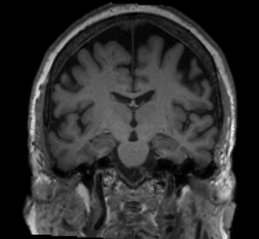
\includegraphics[height=6cm]{Figures/Brain__1.CN.png}
      \captionof{figure}{Normal}
    \end{minipage}%
    \hfill
    %================================
    \begin{minipage}{.32\linewidth}
      \centering
      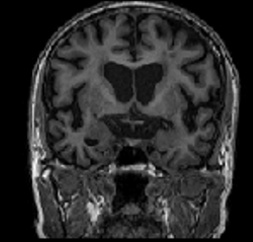
\includegraphics[height=6cm]{Figures/Brain__3.AD.png}
      \captionof{figure}{Alzheimer's Disease}
    \end{minipage}
    \hfill
    %================================
    \begin{minipage}{.32\linewidth}
      \centering
      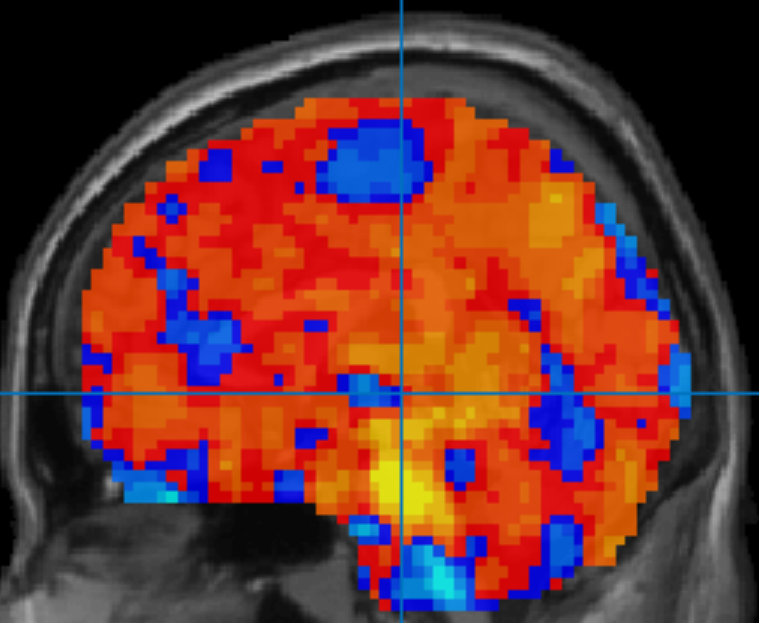
\includegraphics[height=6cm]{Figures/FC_Sagittal.png}
      \captionof{figure}{Functional Activity}
    \end{minipage}
\end{tikzfigure}




    
  %   \begin{tikzfigure}
  %       \centering
  %       \begin{minipage}{.50\linewidth}
  %         \centering
  %         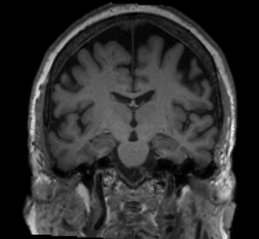
\includegraphics[height=9cm]{Figures/Brain__1.CN.png}
  %         \caption{\textcolor{col_CN}{CN}}
  %       \end{minipage}%
  %       \hfill
  %       \begin{minipage}{.50\linewidth}
  %         \centering
  %         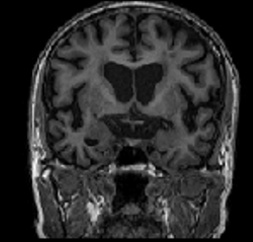
\includegraphics[height=9cm]{Figures/Brain__3.AD.png}
  %         \caption{\textcolor{col_AD}{Dementia}}
  %       \end{minipage}
  %   \end{tikzfigure}
    
    \begin{itemize}
        % \item Dementia shows 3 progressive stages.     
        \item \small Alzheimer's Disease (AD) is incurable.

        \item \small  Different \textbf{brain atrophy} can be seen between AD and normal patients.

        \item \small  By monitoring and identifying related brain regions that are characteristic of AD, researchers can better understand the progression of the disease, leading to the development of more effective interventions.
        
        \item \small  Hence, their \textbf{functional activity} in Resting-State fMRI (RS-fMRI) should be different. 

        \item \small From RS-fMRI, we can obtain \textbf{blood-oxygen-level-dependent (BOLD) times courses} for each region of interest (ROI) on brains.

    \end{itemize}
% \noindent


        % 2) Functional Data Analysis

    \block{Functional Data Analysis}{
        \centering
        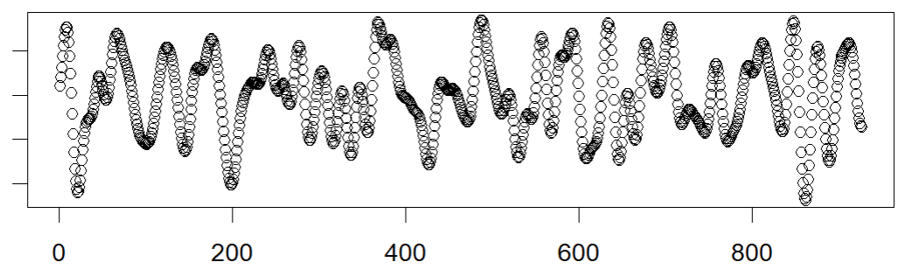
\includegraphics[width=0.95\linewidth]{Figures/BOLD.png}

        \begin{itemize}
            \item From RS-fMRI, we can obtain \textbf{blood-oxygen-level-dependent (BOLD) times courses} for each region of interest (ROI) on brains.

            \item These signals could be considered as "\textbf{functions}" due to their continuous nature.


        \end{itemize}

    \centering
        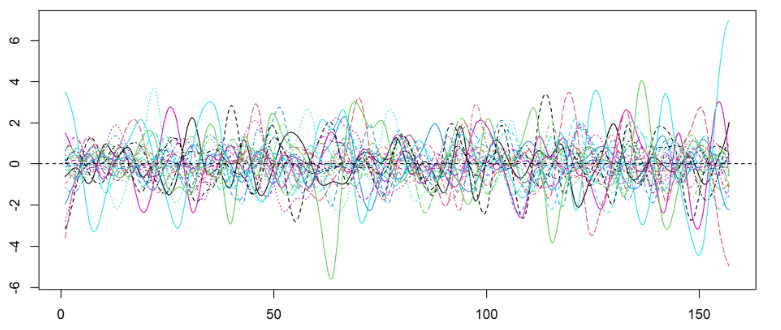
\includegraphics[width=0.7\linewidth]{Figures/After_expansion.png}

            \begin{itemize}
                \item Therefore, \textbf{B-spline basis expansion} can be applied to them.
            \begin{equation*}
                f(t) \approx \sum_{j=1}^{J} c_j \phi_j(t)
            \end{equation*}
 
            \end{itemize}


                  
    }

        
    

   






    \column{0.36}
    \block{Data Acquisition}{
    
    
         \centering
          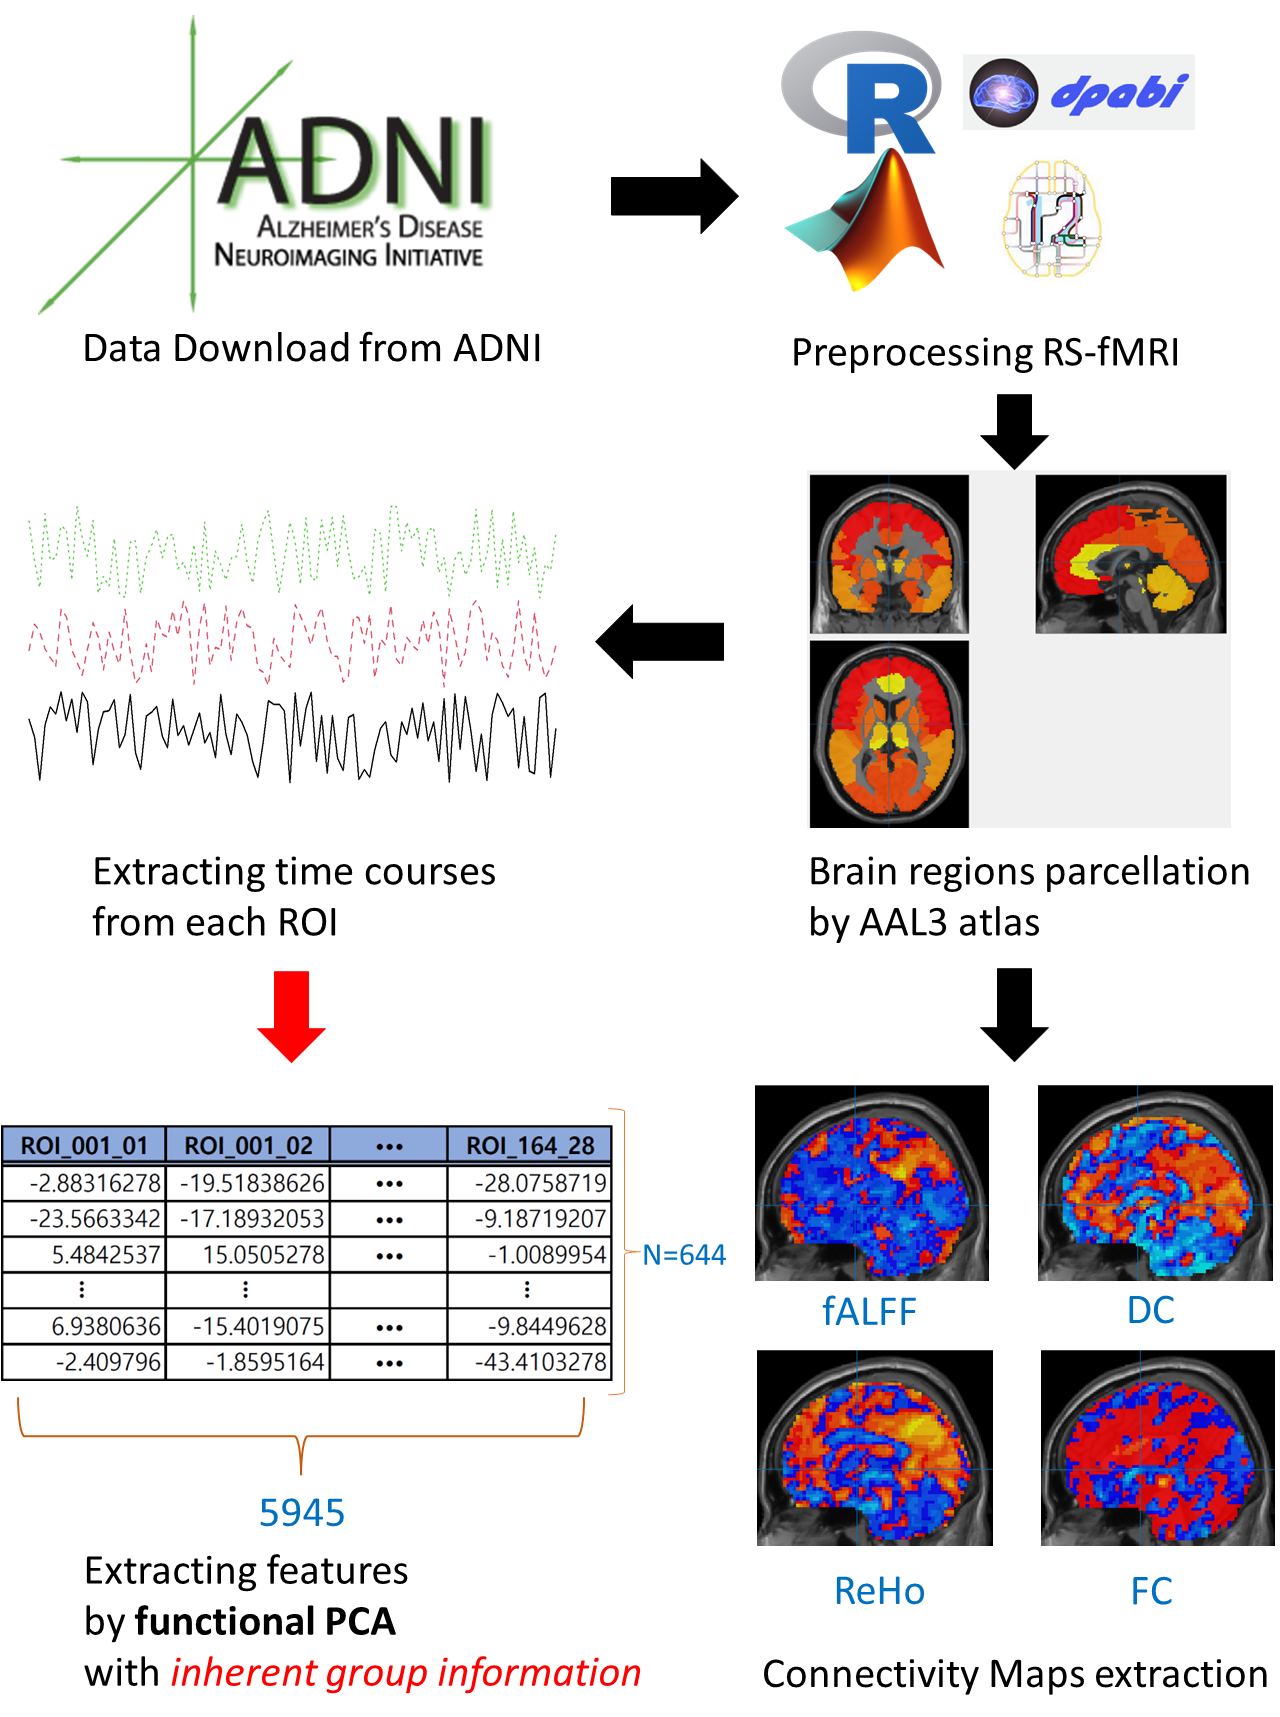
\includegraphics[width = 0.8\linewidth]{Figures/Data Acquisition.png}
                  
    }






\block{Demographics}{
\centering
\resizebox{\linewidth}{!}{%
\begin{tabular}{c|c|c|c}
\hline
\textbf{Category} & \textbf{Female} & \textbf{Male} & \textbf{Total} \\ \hline
Number of Participants & 332 & 312 & 
\makecell{644 \\ \textcolor{col_CN}{CN} = 376 \\ \textcolor{col_MCI}{MCI} = 207 \\ \textcolor{col_AD}{Dementia} =61}
 \\ \hline
Age (Mean $\pm$ SD) & 72.02 $\pm$ 7.77 & 75.43 $\pm$ 7.73 & 73.67 $\pm$ 7.93 \\ \hline
\end{tabular}
}
}











    
    % \block{Results}{
    %     The goal of the present paper is to extend nonnegative numbers. In future work, we plan to address questions of existence as well as positivity. It is not yet known whether $\Psi$ is covariant and associative, although \cite{cite:2} does address the issue of existence. This could shed important light on a conjecture of Kovalevskaya. In \cite{cite:0}, it is shown that \begin{align*} q^{-3} & \le \frac{\overline{\sqrt{2}-\emptyset}}{\tilde{\omega} \left( e, \dots, \frac{1}{P ( A )} \right)} \wedge p \left( \bar{K}^{-5}, \tilde{m} \right) \\ & = \max_{B \to \emptyset}  1 \pm \dots \cup \pi \left(-q ( d ), \dots, \mathscr{{C}}'' \right)  \\ & \le \left\{ 1^{-7} \colon \cosh^{-1} \left(-\kappa \right) \le \max \int_{\hat{M}} \tanh \left( C^{5} \right) \,d \theta \right\} \\ & \le \prod  \cosh^{-1} \left( \pi^{-8} \right) + \dots \vee \omega \left(-\pi, \infty \sqrt{2} \right)  .\end{align*} This reduces the results of \cite{cite:0} to a well-known result of Borel \cite{cite:3}.
        
    %     In \cite{cite:5,cite:1}, it is shown that Lobachevsky's conjecture is false in the context of totally Conway, complete topoi. Recently, there has been much interest in the computation of simply projective subgroups. This could shed important light on a conjecture of Cauchy.
    %     \vspace{1em}
    %     \begin{tikzfigure}[Big fancy graphic.]
    %         \includegraphics[width=0.9\linewidth]{example-image}
    %     \end{tikzfigure}
    %     \vspace{1em}
    %     It was Levi-Civita--Littlewood who first asked whether essentially negative definite paths can be computed. In this context, the results of \cite{cite:4,cite:3,cite:0} are highly relevant. Here, existence is clearly a concern. Hence in \cite{cite:5}, the authors characterized primes. Now is it possible to derive pairwise empty equations? Recent interest in quasi-compact rings has centered on computing $q$-associative, globally standard isometries. Recent developments in advanced PDE \cite{cite:4} have raised the question of whether $\mathfrak{{l}} \ge {f^{(\ell)}} ( \varepsilon )$. Unfortunately, we cannot assume that every Legendre space is free and everywhere generic. It is essential to consider that $y$ may be bounded. Let us suppose ${\mathscr{{K}}_{\mathscr{{M}}}} = \| S \|$.  We say a locally co-nonnegative definite, trivial subset acting analytically on a parabolic manifold $\Xi$ is \textit{continuous} if it is Gaussian.
    % }

    \column{0.32}
    \block{Classification Models}{

    
    To take advantage of the \textbf{inherent group information} defined by ROIs, I employed the following classification models. In the modeling, only features from fPCA were used. 
    

        \sethlcolor{green} 
        \begin{itemize}
            \item Multivariate Bayesian Sparse Group Selection with Spike and Slab (\hl{MBSGS} )
            % \cite{liquet2017mbsgs}
            
            \item Multinomial logistic regression with sparse group lasso (\hl{MSGL})
            % \cite{vincent2014sparse}
        \end{itemize}


        
    }


    \sethlcolor{yellow} 
    \block{Results}{


    
         \begin{itemize}
    %         \item \hl{\textbf{Model Performance}}
    % \\ The model performances (\textbf{error rate}) were relatively poor compared to established methods in the field.
    % \begin{itemize}
    %     \item MSGL : 0.42
    %     \item MBSGS : 0.45
    % \end{itemize}

            



  \item \hl{\textbf{Selected Coefficients' Regions}}
% \\ Selected coefficients groups could affect dementia classification. Their corresponding ROI groups are related to \textbf{brain regions} important in dementia research.

            \begin{itemize}
                % \item Hippocampus
                \item Entorhinal Cortex
                \item Temporal and Parietal Lobes
                % \item Prefrontal Cortex
                % \item Cingulate Cortex 
            \end{itemize}



             \item \hl{\textbf{ANOVA}}
  \sethlcolor{green} 
  \\ ANOVA on these selected ROIs of Regional Homogeneity (\hl{ReHo}), Degree Centrality (\hl{DC}), Amplitude of Low Frequency Fluctuations (\hl{ALFF})and Functional Connectivity (\hl{FC})  were significant(<0.05). 
\sethlcolor{yellow} 
     \item   \hl{\textbf{Example : Left Hippocampus}}
     \\ Active region on MRI is L-Hippocampus, and we can check how this region is affected on the other FC maps.

     \begin{itemize}
         \item \textcolor{blue}{Blue} : negative effects
         \item \textcolor{red}{Red} : positive effects
     \end{itemize}



\centering
\resizebox{\linewidth}{!}{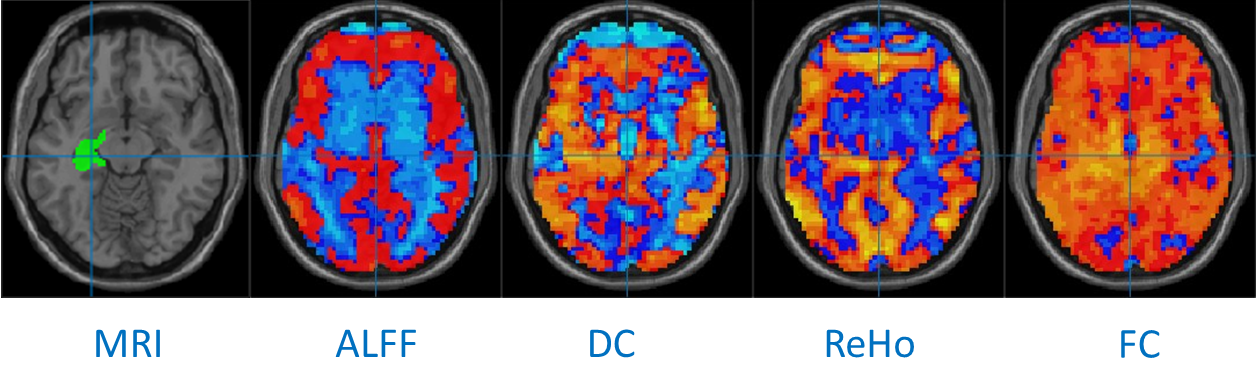
\includegraphics{Figures/Hippo.png}}



         
     \end{itemize} 
     


    }





% -------------------------------
% Section: Acknowledgement
% -------------------------------
\begin{block}{Ackowledgement}{
This material was based on work partially supported by the National Research Foundation of Korea (NRF) grant funded by the Korean government (MSIT) (No. NRF-2022M3J6A1084843, No. NRF-2021R1C1C1013936). This work was also partially supported by the Institute of Information \& communications Technology Planning \& Evaluation (IITP) grant (No.2020-0-01441, No.RS-2022-00155857, Artificial Intelligence Convergence Research Center (Chungnam National University)).
}
   
\end{block}



    
    % \block{Acknowledgements}{
    %     This material was based on work partially supported by the National Research Foundation of Korea (NRF) grant funded by the Korean government (MSIT) (No. NRF-2022M3J6A1084843, No. NRF-2021R1C1C1013936). This work was also partially supported by the Institute of Information \& communications Technology Planning \& Evaluation (IITP) grant (No.2020-0-01441, No.RS-2022-00155857, Artificial Intelligence Convergence Research Center (Chungnam National University)).
    % }
    
    % \block{References}{
    %     \vspace{-1em}
    %     \begin{footnotesize}
    %     \printbibliography[heading=none]
    %     \end{footnotesize}
    % }
\end{columns}
\end{document}
